\section{Introduction}

The overall aim of this project is to perform the task of refining a Finite Element Mesh (FEM), (see section 2.1 for description of FEM) using a hybrid approach which combines stress based method as is traditionally used for FEM refinement with an approach that uses techniques from Artificial Intelligence and Machine Learning. \\

\noindent
Finite Element Analysis (FEA) is a method widely used across different engineering domains to simulate structures under certain conditions. A typical step within the design process for mechanical components involves first designing the component within a CAD application before running a simulation on the design using knowledge of the conditions it is expected to perform under. Having defined the components geometry in continuous terms using CAD software a Finite Element System will break it down into a number of segments (known as elements) which together form a mesh (known as a Finite Element Mesh (FEM). The values of stress within  each of the discrete elements is calculated and then the process of breaking the mesh down into further smaller elements in areas where high levels of stress are encountered, the process is then repeated in an iterative manner until the levels of stress cease to increase or after a defined number of iterations. FEA allows engineers to observe the effect the conditions have on the entire structure, see figure 1. \\ 

\noindent
The success of the project will be determined by implementation of a system that is able to combine the stress and AI based refinement methods in order to refine a mesh of a quality comparable to that of a successful stress based method. Additionally there is benefit in  achieving this quality in less time than the traditional stress based approach. \\ 

\noindent
This Dissertation starts with a review of the FEA process followed by looking at some of approaches that have been taken to refine and evaluate the quality of meshes automatically before continuing to describe the design and discuss challenges of implementing the system. The system is then demonstrated as capable of correctly performing this task in the final evaluation section. \\

\section{Motivation and Background}
During a year long industrial placement at a major aerospace company I worked closely with mechanical engineers, who routinely ran computer programs to calculate the stresses through physical components used in aeronautical designs. The programs used Finite Element Analysis (FEA) to accurately calculate the stresses across the components. However, applying FEA to detailed structures of considerable size can take many hours in execution time to obtain a result. I discovered that it was not uncommon for experienced engineers to correctly predict the regions of high stress revealed by the analysis prior to its completion. This led me to consider how the knowledge of an experienced engineer could be used by an FEA process to reduce the time required to calculate the stress for mechanical components and was consequently the inspiration for the project. \\ 

\noindent
Over the past forty years FEA has emerged as a prominent technology for simulating complex real world engineering problems \cite{cite0, DolsakPaper94}. FEA works by solving a system of differential equations with each equation representing a single element in a geometric mesh. By doing this FEA is able to generate highly accurate approximations for the properties of complex physical systems \cite{DolsakPaper94, IntroductionToFE}. The method can also be highly computationally expensive with the complexity typically increasing exponentially with the model size \cite{DolsakPaper94}. Analysis therefore proves to be highly time consuming and costly for individuals and organisations to conduct \cite{ConsultRuleIntellSystemFE, cite03}.\\


\subsection{Properties of Finite Element Models}
Although this is a computer science dissertation rather than a mechanical engineering dissertation it is still important to briefly outline the general principals and properties that underpin the FEA method in order to have a general appreciation for how the design and evaluation of the final software system was conducted. \\ 

\noindent
Finite Element Models have several key properties that need to be specified by the engineers who create them, the configuration of these properties greatly determine the results obtained from the models execution. The first of these properties that an FE model has is the mesh (known as a Finite Element Mesh or FEM). The mesh is constructed out of nodes, points which act as intersections between the second component- elements which are either a polygon or a polyhedron between the nodes. Nodes and elements are important concepts as they provide the theoretical framework for reasoning about the other properties of a mesh and hence the overall quality of the model \cite{IntroductionToFE}.\\ 

\noindent
Elements within FE models can be different types each defined by their shape. Different shaped elements are selected based on the type of structure that is being assessed and the simulation conditions, some typical examples would be a quadrilateral also known as a quad4 and a triangle (tri3). Appendix B shows the different element types supported by the FE solver (used to calculate stresses in elements) used for this project which is called LISA. \\ 

\noindent
In every type of analysis that the FE method is used for (thermal, structural, fluid flow, electrical) there is a specific differential equation associated with each of the elements. In order to achieve overall convergence of the model the equations must be solved simultaneously to achieve a value for each of the discrete elements \cite{IntroductionToFE}. For this project attention is given specifically to the problem of FEA meshing in the context of static structural analysis where the value calculated across each element is its stress. Stress is defined as force over a given area in an object and arises from some external force being applied. Static structural analysis is one of the most common engineering applications of FEA and has a large  body of research that is relevant to this project. \cite{DolsakPaper94}\cite{IntroductionToFE}.\\

\noindent
In addition to the nodes and elements FE models also contain loads and constraints. Loads can be thought of as the phenomena from the outside world that is acting on the structure and consequently inducing some kind of physical effect on it. Loads are used by engineers to model the conditions which the structure will be expected to perform under when it is manufactured and enters operation. \\

\noindent
Constraints are another fundamental concept that describe where the model is attached to the outside world. When computing stresses through the model there needs to be an area through which the stresses are assumed to leave. FEA is only able to calculate the stresses through the model using the law of conservation of energy i.e. energy cannot be created or destroyed meaning that any energy entering the system as an input such as force needs a means by which to leave it, the constraint. \\

\noindent
For example in figure 6 showing a suspension bridge model, the simulation is to be run with the forces induced upon the cables and the towers in the negative x direction as represented by the green vectors. The corresponding constraint area through which the force must leave is specified as the base of each bridge pillar and represented by multiple red arrows on each corresponding corner.\\

\noindent
The final piece of information needed in order to calculate the stresses through the model is material data. Material data is associated with the models elements and is usually defined using two main parameters which are:

\begin{itemize}
\item Youngs Modulus - The ratio of stress over strain for a given material, i.e. for an amount of internal force endured by a material how much does it deform, a material such as rubber therefore has a low value for Young's modulus while diamond has a high value \cite{YoungsModulus}.

\item Poissons ratio - Amount of deformation that occurs perpendicular to the force that is applied to the material \cite{PossionsRatio}. 
\end{itemize}

\noindent
For the sake of simplicity all structures used to evaluate the final software solution have assumed steel as their material property. Steel is a common material used within manufacturing of many mechanical components and does not exhibit any abnormal properties. This is beneficial for evaluation as it removes variability in the results that could arise from selecting a more complex material. The system I have designed would also work with these more complex materials however the process of assessing the results could potentially be much harder without a more extensive engineering background and better knowledge of the specific materials. 

\subsection{Limitations and general considerations}
\noindent
An important consideration when conducting FEA is the trade-off of a model's accuracy against the time it takes for the solver to perform an analysis of the model. A major variable determining this trade-off is the model's mesh structure which discretizes the problem so that a simulation can be run on it. A mesh that is finer is more computationally expensive but also produces results of greater accuracy. It is therefore desirable to generate a mesh which is fine where accuracy is most needed but coarse where it is not \cite{cite04}. \\


\noindent
For engineers the value obtained through computing the stresses under a particular set of conditions is feedback on the quality of their design. Ideally the results from an analysis will provide a good understanding of where the design is weak and how concentrated this weakness is. This information is used to either help verify the designs' quality or alternatively inform changes to its geometry or material properties so as to reduce stress on subsequent analysis \cite{cite06}.\\

\noindent
To understand the gradient of stress within a part of the model the mesh needs to be designed carefully. As each element can only display values calculated from its edge nodes a smooth gradient requires a higher concentration of elements in areas under higher stress. A high quality mesh is therefore considered to have a higher concentration of elements in areas of predicted high stress while retaining lower concentration elsewhere, thereby revealing weaknesses in the design while minimising the models runtime.\\

\noindent
Traditionally the automated mesh refinement process consists of computing stresses for a model with an initial coarse mesh and low computation cost, once rough stresses have been computed the elements in areas of higher stress can be divided recursively into additional elements in order to achieve smoother gradients on further executions \cite{cite03}. Figure 1 shows a mesh which has been refined in an area of higher stress thus providing a clearer indication of a components weakness. \\ 

\noindent
Unfortunately for many large models this method for refining a mesh is still excessively costly \cite{DolsakPaper91}. It is therefore worth investigating use of alternative approaches posed by the field of computer science and artificial intelligence that could support the traditional high stress meshing approach. \\ \\ \\ \\

\begin{figure}[H]
  \centerline{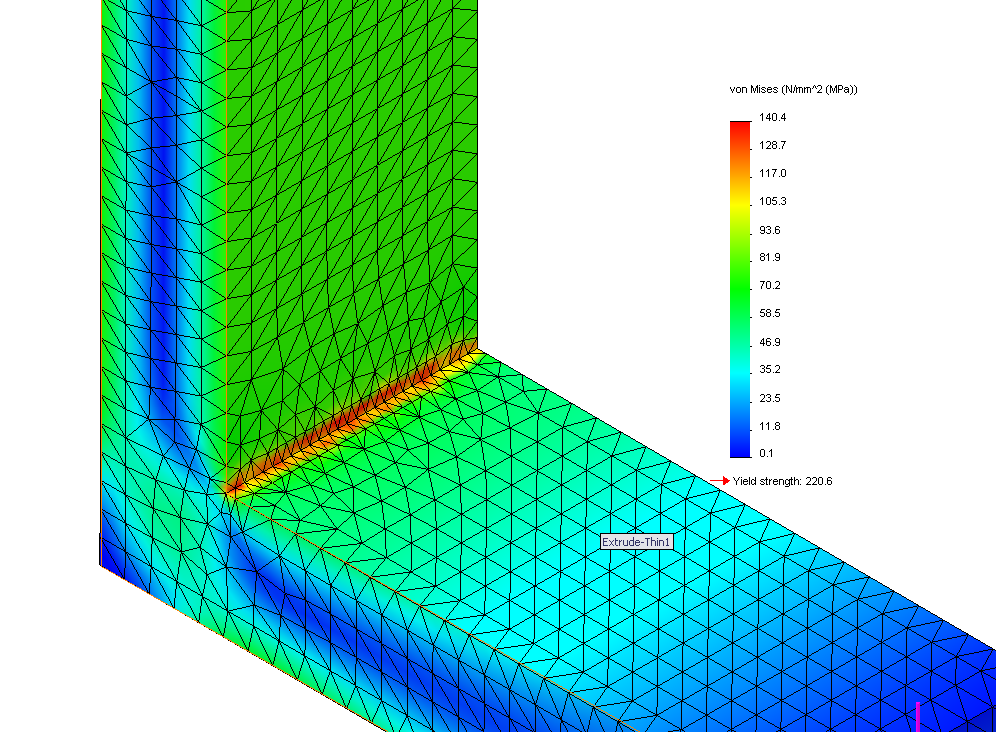
\includegraphics[width=150mm, scale=0.5]{../Graphics/StressedCorner.png}}
  \caption{Mesh refinement in corner under high stress image source: (\cite{HighStressCorner})}
  \label{fig:boat1}
\end{figure}